\documentclass{beamer}
\usetheme{Berkeley}
\usecolortheme{sidebartab}
\usepackage{multimedia}
\usepackage{pgf,pgfarrows,pgfnodes}
\usepackage{multicol}
\usepackage{cite}
\usepackage{lmodern}
\usepackage{hyperref}

\logo{\includegraphics[height=1.45cm]{uvmlogo.png}}

%\usepackage[cmex10]{amsmath}   
%\usepackage{graphicx}

\author[Owen Myers]{Owen Myers \and Junru Wu \and Jeff Marshall}

\date{\today}

\title{Chaos in the Electric Curtain}

\institute{University of Vermont\\Funded by NASA Kennedy (Dr. Carlos Calle)}

\begin{document}


\maketitle

%-----------------------------------------------------------------------------------------
%-----------------------------------------------------------------------------------------
%\section{Outline}
%\begin{frame}{Outline}
%    \begin{itemize}
%        \item What is the Electric Curtain? 
%        \item Computational Methods and Simplifications
%        \item The 1D Electric Curtain (surface particle motion) 
%        \item The 2D Electric Curtain (off surface motion) 
%    \end{itemize}
%\end{frame}
%-----------------------------------------------------------------------------------------
%-----------------------------------------------------------------------------------------

\section{The Standing Wave Electric Curtain}

\subsection{Background}

\begin{frame}{The Electric Curtain}

    %\centering
        
    \begin{pgfpicture}{0cm}{0cm}{10cm}{6cm}

    %rectangles
    \pgfrect[stroke]{\pgfpoint{0cm}{1cm}}{\pgfpoint{8cm}{2cm}}
    \pgfrect[stroke]{\pgfpoint{2cm}{4cm}}{\pgfpoint{8cm}{2cm}}

    %corner lines
    \pgfline{\pgfxy(0.0,3.0)}{\pgfxy(2.0,6.0)}
    \pgfline{\pgfxy(8.0,3.0)}{\pgfxy(10.0,6.0)}
    \pgfline{\pgfxy(8.0,1.0)}{\pgfxy(10.0,4.0)}
    \pgfline{\pgfxy(0.0,1.0)}{\pgfxy(2.0,4.0)}

    %first circles
    \pgfcircle[stroke]{\pgfpoint{0.5cm}{2cm}}{.1cm}
    \pgfcircle[stroke]{\pgfpoint{1.5cm}{2cm}}{.1cm}
    \pgfcircle[stroke]{\pgfpoint{2.5cm}{2cm}}{.1cm}
    \pgfcircle[stroke]{\pgfpoint{3.5cm}{2cm}}{.1cm}
    \pgfcircle[stroke]{\pgfpoint{4.5cm}{2cm}}{.1cm}
    \pgfcircle[stroke]{\pgfpoint{5.5cm}{2cm}}{.1cm}
    \pgfcircle[stroke]{\pgfpoint{6.5cm}{2cm}}{.1cm}
    \pgfcircle[stroke]{\pgfpoint{7.5cm}{2cm}}{.1cm}

    %second circles 
    \pgfcircle[stroke]{\pgfpoint{2.5cm}{5cm}}{.1cm}
    \pgfcircle[stroke]{\pgfpoint{3.5cm}{5cm}}{.1cm}
    \pgfcircle[stroke]{\pgfpoint{4.5cm}{5cm}}{.1cm}
    \pgfcircle[stroke]{\pgfpoint{5.5cm}{5cm}}{.1cm}
    \pgfcircle[stroke]{\pgfpoint{6.5cm}{5cm}}{.1cm}
    \pgfcircle[stroke]{\pgfpoint{7.5cm}{5cm}}{.1cm}
    \pgfcircle[stroke]{\pgfpoint{8.5cm}{5cm}}{.1cm}
    \pgfcircle[stroke]{\pgfpoint{9.5cm}{5cm}}{.1cm}

    %lines on left of circles
    \pgfline{\pgfxy(0.4,2)}{\pgfxy(2.4,5)}
    \pgfline{\pgfxy(1.4,2)}{\pgfxy(3.4,5)}
    \pgfline{\pgfxy(2.4,2)}{\pgfxy(4.4,5)}
    \pgfline{\pgfxy(3.4,2)}{\pgfxy(5.4,5)}
    \pgfline{\pgfxy(4.4,2)}{\pgfxy(6.4,5)}
    \pgfline{\pgfxy(5.4,2)}{\pgfxy(7.4,5)}
    \pgfline{\pgfxy(6.4,2)}{\pgfxy(8.4,5)}
    \pgfline{\pgfxy(7.4,2)}{\pgfxy(9.4,5)}

    %lines on right of circles
    \pgfline{\pgfxy(0.6,2)}{\pgfxy(2.6,5)}
    \pgfline{\pgfxy(1.6,2)}{\pgfxy(3.6,5)}
    \pgfline{\pgfxy(2.6,2)}{\pgfxy(4.6,5)}
    \pgfline{\pgfxy(3.6,2)}{\pgfxy(5.6,5)}
    \pgfline{\pgfxy(4.6,2)}{\pgfxy(6.6,5)}
    \pgfline{\pgfxy(5.6,2)}{\pgfxy(7.6,5)}
    \pgfline{\pgfxy(6.6,2)}{\pgfxy(8.6,5)}
    \pgfline{\pgfxy(7.6,2)}{\pgfxy(9.6,5)}

    \begin{pgfscope}
        \pgfsetlinewidth{1pt}
        %long vertical wire lines
        \pgfline{\pgfxy(0.5,1.9)}{\pgfxy(0.5,.4)}
        \pgfline{\pgfxy(2.5,1.9)}{\pgfxy(2.5,.4)}
        \pgfline{\pgfxy(4.5,1.9)}{\pgfxy(4.5,.4)}
        \pgfline{\pgfxy(6.5,1.9)}{\pgfxy(6.5,.4)}


        %short vertical wire lines 
        \pgfline{\pgfxy(1.5,1.9)}{\pgfxy(1.5,1.5)}
        \pgfline{\pgfxy(3.5,1.9)}{\pgfxy(3.5,1.5)}
        \pgfline{\pgfxy(5.5,1.9)}{\pgfxy(5.5,1.5)}
        \pgfline{\pgfxy(7.5,1.9)}{\pgfxy(7.5,1.5)}

        %conecting wires
        \pgfline{\pgfxy(1.5,1.5)}{\pgfxy(8.9,1.5)}
        \pgfline{\pgfxy(0.5,0.4)}{\pgfxy(8.9,0.4)}
    \end{pgfscope}

    %power source circles
    \pgfcircle[stroke]{\pgfpoint{9.4cm}{.4cm}}{.5cm}
    \pgfcircle[stroke]{\pgfpoint{9.4cm}{1.5cm}}{.5cm}

    %AC squigles
    \pgfmoveto{\pgfxy(8.9,1.5)}
    \pgfcurveto{\pgfxy(9.4,.8)}{\pgfxy(9.4,2.2)}{\pgfxy(9.9,1.5)}
    \pgfstroke

    \pgfmoveto{\pgfxy(8.9,0.4)}
    \pgfcurveto{\pgfxy(9.4,1.1)}{\pgfxy(9.4,-.3)}{\pgfxy(9.9,.4)}
    \pgfstroke

    %Anotations
    \pgfputat{\pgfxy(1.2,6.45)}{\pgfbox[center,center]{$Dielectric$ $Surface$}}
    \pgfputat{\pgfxy(2.9,5.5)}{\pgfbox[center,center]{$Electrodes$}}

    

    \end{pgfpicture}


\end{frame}


%********************************************************************
%\begin{frame}
%    The electric curtain was Patented in 1974 by Senichi Masuda for particle manipulation in an
%    electrostatic powder painting booth (Masuda, 1974).\\
%    Major application interests include dust mitigation in extraterrestrial environments (Mazumder et
%    al., 2007) and various particulate separation applications including:
%    \begin{itemize}
%        \item[-] separation of cells in solution (Masuda et al., 1988)
%        \item[-] separation of by-products from agricultural processes (Weiss et al., 1984)
%        \item[-] separation of particles with different charge to mass ratios (Kawamoto, 2008)
%    \end{itemize}
%\end{frame}
\subsection{Why Study Chaos?}
\begin{frame}{Why Study the Electric Curtain's Chaotic Dynamics}
    \begin{columns}
        \begin{column}{5cm}
            \movie[width=5cm,height=4cm,loop,poster]{}{032411n2-1.avi}
        \end{column}
        \begin{column}{5cm}
        \footnotesize
            A better understanding of the sensitivity of particle motion to physical parameters will
            improve applications such as:
        \begin{itemize}
            \item[-] Dust mitigation in extraterrestrial envirionments (Mazumder et al., 2007)
            \item[-] Separation of cells in solution (Masuda et al., 1988)
            \item[-] Separation of by-products from agricultural processes (Weiss et al., 1984)
            \item[-] Separation of particles with different charge to mass ratios (Kawamoto, 2008)
        \end{itemize}
      
        \end{column}
    \end{columns}
\end{frame}



%********************************************************************
\section{Computational Methods}

\begin{frame}{Simplifications}
    \begin{columns}
        \begin{column}{4.5cm}
            \movie[width=4.5cm,height=2.5cm,loop,poster]{}{periodTwo.avi}\\
            \movie[width=4.5cm,height=2.5cm,loop,poster]{}{2Dmovie.avi}
        \end{column}
        \begin{column}{6cm}
            \begin{enumerate}
                \scriptsize
                \item Primarily investigated single particle motion on the surface of the EC (1D) model.
                \item Only preliminary work on particle motion above the surface.
                \item In both cases dissipative forces are considered.
                \item[-] 1D Dissipative forces: Rolling resistance and viscous fluid force.
                Both are proportional to velocity (Brillianttov and Poschell, 1999).
                \item[-] 2D: Viscous fluid force (non-dissipative collisions) 
                \item For the center line charge approximation the electrodes are considered as one  
                dimensional wires. To make this approximation valid we need the surface to be an
                adequate distance above the plane of electrodes.
            \end{enumerate}
        \end{column}
    \end{columns}
\end{frame}

\subsection{Electric Field Approximation}

\begin{frame}{Center Line Charge Approximation}
    Approximate electric field equations (Masuda and Kamimura, 1975):
    %conformal transformation from a sum of an infinite series
    \[
    E_x=\frac{k Q}{4\pi\epsilon_0} \sum_{n=0}^{1} \frac{\sin(k x - n \pi) \cos(\omega t - n
        \pi)}{\cosh(k y) - \cos(k x - n\pi)}
    \]
    
    \[
    E_y = \frac{k Q}{4\pi\epsilon_0}\sum_{n=0}^{1} \frac{\sinh(k y) \cos(\omega t-n\pi)}
        {\cosh(k y)-\cos(k x - n\pi)}
    \]

\end{frame}

%coment this out because it is not nesasary given the amount of time i have
%\begin{frame}{Equations of Motion}
%
%    Full equations of motion
%
%    \[
%    \frac{d^2x}{dt^2}+\frac{\beta}{m}\frac{dx}{dt}=
%        \sum_{n=0}^{1} J \frac{\sin(k x - n\pi ) \cos(\omega t - n\pi)}{\cosh(k y) - \cos(k x - n\pi)} 
%    \]
%
%    \[
%    \frac{d^2y}{dt^2} +\frac{\beta}{m}\frac{dy}{dt}=
%        \sum_{n=0}^{1} J \frac{\sinh(k y) \cos(\omega t-n\pi)}{\cosh(k y)-\cos(k x-n\pi )}-g 
%    \]
%    
%    Where $J=kqQ/4m\pi\epsilon_0$ (Interaction Amplitude)
%
%\end{frame}

\begin{frame}{Non-Dimensionalized Parameters}
    \begin{multicols}{2}
        \begin{itemize}
            \item[] $t' = \omega t$
            \item[] $x' = k x$
            \item[] $y' = k y$
            \item[] $j = \frac{k^2 q Q}{4 \pi \epsilon_0 m^2 \omega^2}$
            \item[] $g' = \frac{g k}{\omega^2}$
            \item[] $\beta' = \frac{\beta}{m \omega}$
        \end{itemize}
    \end{multicols}
    
    $j$ is the dimensionless interaction amplitude.

    Dimensionless Equations of Motion:

    \[
    \frac{d^2x'}{dt'^2}+\beta'\frac{dx'}{dt'}= \sum_{n=0}^{1} j \frac{\sin(x' - n\pi ) \cos(t' -
        n\pi)}{\cosh(y') - \cos(x' - n\pi)} 
    \]
    \[
    \frac{d^2y'}{dt'^2} +\beta'\frac{dy'}{dt'}=
        \sum_{n=0}^{1} j \frac{\sinh(y') \cos(t' - n\pi)}{\cosh(y')-\cos(x' - n\pi )}-g' 
    \]
\end{frame}

%\begin{frame}{Setting the Parameters}
%    \begin{enumerate}
%        \item The non-Dimensionalization $x'=kx$ makes the system periodic in space over $0\leq x' \leq 2\pi$. 
%        \item Therefore the electrode spacing is $\pi$ and setting $y'=1$ puts the surface sufficiently
%        far from the electrodes.
%        \item The non-Dimensionalization  $t'=\omega t$ makes the system periodic in time over $0\leq t' \leq 2\pi$.
%    \end{enumerate}
%\end{frame}

\begin{frame}{Interaction Amplitude Regimes}
    Place particle directly above electrode to solve for when the electrostatic force equals the
    gravitational force.
    \[
     \sum_{n=0}^{1} j \frac{\sinh(y') \cos(t' - n\pi)}{\cosh(y')-\cos(x' - n\pi )}=g' 
    \]
    The inequality:
    \[
    \frac{j}{g'}\leq \frac{\cosh^2(y')-1}{2 \cos(t')\cosh(y')}
    \]
    needs to be satisfied for the particle to remain on the surface. When we make $\cos(t')$ one and
    put it $y'=1$ we find that:
    \[
    \frac{j}{g'}\approx .448
    \]
    is the critical ratio that needs to be considered.
\end{frame}


\section{The One Dimensional Electric Curtain}
%\begin{frame}{First-order autonomous equations}
%    \begin{itemize}    
%        \item[] $\dot{x}_1 = x_2$
%        \item[] $\dot{x}_2 = \sum_{n=0}^{1} j \frac{\sin(k' x_1 - n\pi) \cos(x_3 - n \pi)} {\cosh(k' y') - \cos(k' x - n\pi)} - \beta'x_2$
%        \item[] $\dot{x}_3 = 1$ 
%    \end{itemize}
%    where $x_3=t$
%\end{frame}

\begin{frame}{The full periodic phase space}
    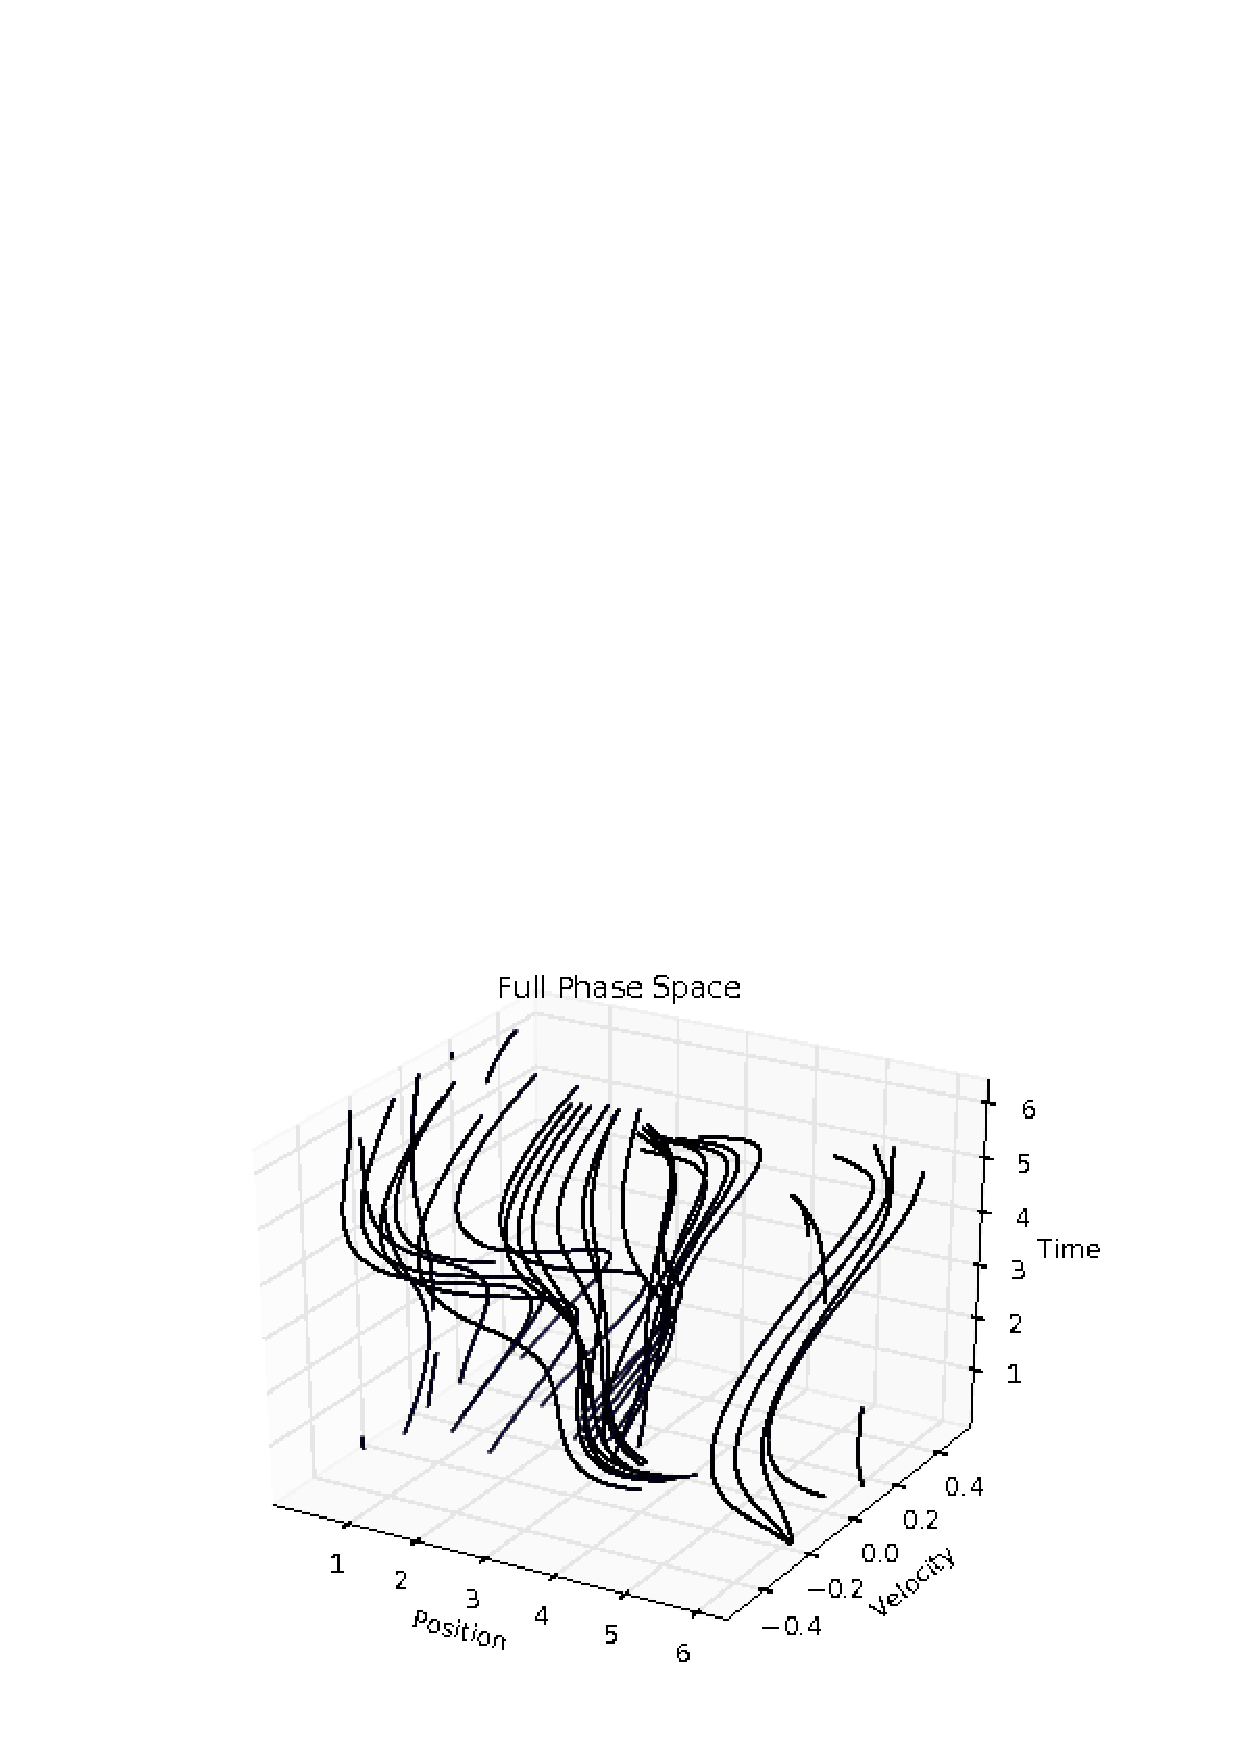
\includegraphics[scale = 0.5]{fullphasespaceEX.png}
\end{frame}

\subsection{Poincare Sections}
\begin{frame}{Full phase space time sliced}
    \includegraphics[scale = 0.5]{1DtimeSL.png}
\end{frame}

%\begin{frame}{The shifting manifold}
%\end{frame}


\subsection{Bifurcations}
\begin{frame}{Period doubling?}
    \begin{columns}
        \begin{column}{5cm}
            \includegraphics[scale = 0.25]{firstbif.png}
        \end{column}
        \begin{column}{5cm}
            Period 2 Orbit\\
            \movie[width=5cm,height=2.5cm,loop,poster]{}{periodTwo.avi}
            Period 4 Orbit\\
            \movie[width=5cm,height=2.5cm,loop,poster]{}{periodFour.avi}
        \end{column}
    \end{columns}
\end{frame}


\begin{frame}{A unique period doubling rout to chaos}
    \begin{columns}
        \begin{column}{5cm}
            \includegraphics[scale = 0.25]{secondbif.png}
            \\
            \includegraphics[scale = 0.25]{thirdbif.png}
        \end{column}
        \begin{column}{6cm}
            Chaotic Orbit
            \movie[width=6cm,height=2.1cm,loop,poster]{}{chaos.avi}
        \end{column}
    \end{columns}
\end{frame}


\section{Two Dimensional Electric Curtain}
\begin{frame}{Preliminarly 2D Work}
    \begin{columns}[t]
        \begin{column}{5cm}
            \includegraphics[scale = 0.2]{2Dxslice.png}
        \end{column}
        \begin{column}{5cm}
            \includegraphics[scale = 0.2]{2Dyslice.png}
        \end{column}
    \end{columns}
\end{frame}

%\begin{frame}{Acknowledgments}
%    \begin{itemize}
%        \item[-] This work has been supported by NASA under cooperative agreement number NNX08AZ07A.\\
%        \item[-] I would also like to thank junru wu and jeff marshall for all of their help and suport:
%    \end{itemize}
%    \begin{columns}
%        \begin{column}{4cm}
%            \includegraphics[scale = .65]{wu.png}
%            \tiny{Junru Wu}
%        \end{column}
%        \begin{column}{4cm}
%            \includegraphics[scale = .4]{jeff.png}
%            \tiny{Jeff Marshall}
%        \end{column}
%    \end{columns}
%\end{frame}
\section{Conclusion}
\begin{frame}{Conclusion}
    \begin{itemize}
        \item We have analyzed a simplified model of the electric curtain by using
        Poincar$\acute{e}$ sections and bifurcation diagrams. 
        \item Particle trajectories in a real Electric curtain have the potential to be
        chaotic but may also exhibit order. Understanding the chaotic dynamics may help improve the
        electric curtain for its current applications and may suggest the possibility of new applications.
        \item \textbf{Future work:}
        \item[-] Improve our computational model and start to include particle-particle interactions.
        \item[-] Experimentally verify our computational findings.
        \item[-] Quantify the strength of chaos (find the Lyapunove spectrum)
    \end{itemize}
\end{frame}

\begin{frame}{Bibliography}
\tiny
    \begin{itemize}
    \item[] S. Masuda, "Booth for electrostatic powder painting with contact type electric field curtain,"
    USA Patent 3801869, April, 1974.\\

    \item[] M. Mazumder, R. Sharma, A. Biris, J. Zhang, C. Calle, and M. Zahn, "Self-cleaning transparent
    dust shields for protecting solar panels and other devices," \textit{Particulate Science and
    Technology}, vol. 25, pp. 5-20, May 2007.\\

    \item[] S. Masuda, M. Washizu, and I. Kawabata, "Movement of blood cells in liquid by nonuniform
    traveling field," \textit{IEEE Transactions on Industry Applications}, vol. 24, pp. 217-222,
    Mar/Apr 1998.\\

    \item[] L.C. Weiss and D.P. Thibodeaux, "Separation of seed by-products by an AC electric field,"
    \textit{JAOCS}, vol. 61, no. 5, pp. 886-890, May 1984.\\

    \item[] H. Kawamoto, "Some techniques on electrostatic separation of particle size utilizing
    electrostatic traveling-wave field," \textit{Journal of Electrostatics}, vol. 66, pp. 220-228,
    2008.

    \item[] S. Masuda and T. Kamimura "Approximate methods for calculating a non-uniform traveling
    field," \textit{Journal of Electrostatics}, vol. 1, pp. 351-370, January 1975.
    \end{itemize}
\end{frame}

%\begin{frame}{Bibliography}
%    \bibliographystyle{plainnat}
%    \bibliography{myrefs}
%\end{frame}


%%A displayed formula:
%
%\[
%    \int_{-\infty}^\infty e^{-x^2} \, dx = \sqrt{\pi}
%\]
%An intemized list:
%\begin{itemize}
%    \item itemized item 1
%    \item itemized item 2
%    \item itemized item 3
%\end{itemize}
%
%\begin{theorem}
%    In a right triagle, the square of hypotenuse equals the sum of squares of two other sides.
%\end{theorem}

\end{document}
